% =====================================================================
% Chapter 4: Key Ideas
%
% Required topic: the description of the methodology, at the level of
% the ideas. Chapter 5 defines the same techniques formally.
%
% The text is the Key Ideas section of the paper, word for word. Only
% the structure is adapted: the section becomes a chapter and its four
% paragraphs become sections, and the figure is taken from graphics/.
% =====================================================================
\chapter{Key Ideas}
\label{ch:key-ideas}

In this chapter, we present our key ideas for accelerating the exact analysis of the maximal non-robust bound.
We describe the conditional-triangle relaxation, the perturbation-difference interval, zonotope bound tightening, and incremental verification.

\begin{figure}[t]
\centering
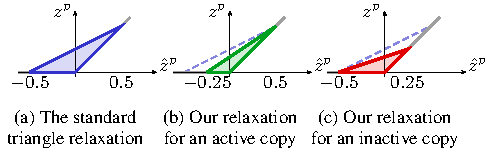
\includegraphics{fig_condtriangle}
\caption{Our triangle relaxation over the input $[-0.5, 0.5]$.}
\label{fig:condtriangle}
\end{figure}

\section{Conditional-Triangle Relaxation}
\label{sec:key-ideas-condtri}

In local robustness, where a single copy of a network is analyzed, the triangle
relaxation has been used extensively to bound a
ReLU's computation through linear constraints~\cite{ehlers2017,singh2019,tjandraatmadja2020convex}.
While we could apply it directly to each of our two copies, it
would lose too much precision and not capture their relation. We propose a novel triangle relaxation that explicitly relies on the relation between a neuron $z_{m,k}$
and its copy $z^{p}_{m,k}$. It has three cases. First, if the triangle over-approximation error of both neuron copies is at most a threshold $\tau$, \tool
relaxes $z_{m,k}$ and $z^{p}_{m,k}$, each with a triangle, and couples them through an interval
bounding their difference. Second, if only
one copy is unstable and its error is at most $\tau$, \tool relaxes it with a triangle. Third, if both copies are unstable and only one has error at most $\tau$, our relaxation encodes
the copy whose error exceeds $\tau$ exactly, say $z_{m,k}$, in particular its activation state (active or inactive) is captured through
a variable or constraint, and replaces the exact encoding of the other copy, $z^p_{m,k}$, with a triangle
\emph{conditioned} on the activation state of $z_{m,k}$ (without knowing that state upfront). This
dynamically captures a more precise triangle.
If both errors exceed $\tau$, \tool encodes both copies exactly.
To illustrate, consider $z^p_{m,k}$ bounded in $[-0.5, 0.5]$, whose standard triangle is the blue one
in Figure~\ref{fig:condtriangle}(a). Assume the two copies' inputs differ by $\hat{z}_{m,k} - \hat{z}^p_{m,k} \in [-0.25, 0.25]$. If
$z_{m,k}$ is active (i.e., $\hat{z}_{m,k} > 0$), then $z^p_{m,k}$'s input is confined to $[-0.25, 0.5]$
and its triangle tightens to the green one in Figure~\ref{fig:condtriangle}(b). If
$z_{m,k}$ is inactive, the input is bounded in $[-0.5, 0.25]$ and its triangle tightens to the red one
in Figure~\ref{fig:condtriangle}(c). Both triangles are half the area of the blue triangle.

\section{Perturbation-Difference Interval}
\label{sec:key-ideas-pert-diff}

Several works over-approximate the difference between two networks with difference intervals, but only
between \emph{distinct} networks~\cite{paulsen2020reludiff,paulsen2020neurodiff,kabaha2025lucid}. We
present perturbation-difference intervals that bound how far apart the clean and perturbed copies are at
each neuron, for popular perturbations such as $\ell_\infty$, brightness, contrast, patch, occlusion,
translation, and rotation, with a single forward pass. We use these intervals not for over-approximation, which loses precision since intervals ignore neuron
dependencies, but as constraints in our constraint-based verifier, and as input to the
conditional-triangle relaxation, as described above. For most perturbations, a pixel's perturbed value depends only on that pixel, so its difference follows
directly from the perturbation, e.g., $[-\ep,\ep]$ under an $\ell_\infty$ perturbation of size $\ep$. For translation and rotation, however, a pixel's perturbed value is
drawn from other pixels, so bounding each pixel's difference in isolation ignores the perturbation's
dependencies and over-approximates it to a useless $[-1,1]$, the maximal difference between two unknown
pixels in $[0,1]$. Since these transform the input linearly, we instead express the difference between
the two copies as a linear function of the shared input and bound it jointly over the pixels it combines.


\section{Zonotope Bound Tightening}
\label{sec:key-ideas-zonotope}

Exact verifiers use the per-neuron intervals $[l_{m,k},u_{m,k}]$ and $[l^{p}_{m,k},u^{p}_{m,k}]$ to
identify the linear neurons $z_{m,k}$ and $z^{p}_{m,k}$, which reduce the complexity of solving the
encoding. We propose to tighten these bounds with a \emph{zonotope}, a popular abstract domain for over-approximating
networks in local robustness~\cite{gehr2018,singh2018fast,singh2019,mirman2018differentiable} and
recently proposed for certifying global robustness~\cite{athavale2026differential}. Unlike that certification, which speeds up verification at the cost of precision, \tool adds the
zonotope only to tighten $[l_{m,k},u_{m,k}]$ and $[l^{p}_{m,k},u^{p}_{m,k}]$, making more neurons linear or near-decided
(enabling our relaxation), without sacrificing precision, which would flag more
inputs as non-robust. Note that our zonotope abstraction complements the perturbation-difference interval: it bounds the
\emph{values} of each neuron rather than the \emph{difference} between the two copies.
For example, consider inputs $x_1, x_2 \in [0,1]$, followed by two first-layer neurons
$z_{1,1} = \mathrm{ReLU}(x_1 - x_2)$ and $z_{1,2} = \mathrm{ReLU}(x_1 + x_2 + 1)$, and a second-layer
neuron $\hat{z}_{2,1} = z_{1,2} - 2z_{1,1}$. Encoding them as a zonotope sets $x_i = 0.5 + 0.5\eta_i$, giving a stable
$z_{1,2} = 2 + 0.5\eta_1 + 0.5\eta_2$ and an unstable
$z_{1,1} = 0.25 + 0.25\eta_1 - 0.25\eta_2 + 0.25\eta_3$, computed with the ReLU transformer~\cite{singh2018fast}. In $\hat{z}_{2,1}$ the shared $\eta_1$ cancels
($0.5 - 2 \cdot 0.25 = 0$), giving $\hat{z}_{2,1} \in [0,3]$, which is stable: $z_{2,1} = \hat{z}_{2,1}$,
encoded with linear constraints. Approximating instead with intervals, as is common, treats
$z_{1,1} \in [0,1]$ and $z_{1,2} \in [1,3]$ independently, giving $\hat{z}_{2,1} \in [-1,3]$ and making
$z_{2,1}$ non-linear, which increases the encoding's complexity.

\section{Incremental Verification}
\label{sec:key-ideas-incremental}

Incremental verification has been shown to scale analysis across applications, in particular local
robustness~\cite{ugare2023,ugare2022fanc,fischer2022,olive2025}. To the best of our knowledge, \tool is
the first to support it for global robustness, transferring the analysis results of a previously
verified network $\Npre$ to a retrained or fine-tuned version $N$ (or a quantized one) that keeps its architecture. It reuses
$\Npre$ in two ways. First, a difference zonotope bounds how far each of $N$'s pre-activations strays
from $\Npre$'s. Since $\Npre$'s bounds are already verified, \tool shifts them by this stray and
intersects the result with $N$'s zonotope bounds, tightening them. Second, \tool warm-starts $N$'s search from $\Npre$'s solution, hinting each unstable neuron's phase
from $\Npre$'s decision where the two networks likely agree. Warm-starting helps in exact verification
since each non-linear neuron splits the search into two, giving exponentially many phase assignments.
Starting from a full or partial one may speed up the search if it matches the optimal solution's phases. As a hint only guides
the solver's branching and can be overturned, it directs the search without sacrificing precision.
For example, assume $\Npre$'s maximal non-robust bound $\hat{\delta}_{c_t}$ is achieved by an input $x$
under which a neuron's pre-activation $\hat{z}^{\mathrm{pre}}_{m,k} = 0.15$, hence active. If $N$'s pre-activation differs from it by a value in
$[-0.25,0.25]$, then $\hat{z}_{m,k} \in [-0.1,0.4]$. Four fifths of this range is positive, so \tool
hints $z_{m,k}$ active. Had it been $[-0.4,0.1]$, it would hint inactive.
